\chapter{Lektion 3}
\section{Kapitel 7}
Som verden udvikler sig ændre efterspørgselen sig på forskellige ting, og dermed ændre antallet og diversiteten af sælgere i forskellige markeder sig også hele tiden. Denne ændring sker når det fx bedre kan betale sig at sælge noget andet(offeromkostninger stiger).

\subsection{The central role of economic profit}
\subsubsection{Three types of profit}
\textbf{regnskabsmæssig profit} er indtjening minus eksplicitte(løn) omkostninger. Det er denne profit firmaer bruger i deres årlige rapporter. 

\textbf{Økonomisk profit} er indtjeningen minus de implicitte(offeromkostninger) og eksplicitte omkostninger, hvilket er offeromkostningerne for alle ressourcerne leveret af firmaets ejer. Hvis denne bliver negativ kaldes det et \textbf{økonomisk tab}. Hvis et firma skal blive på markedet på lang sigt skal det økonomiske overskud være over eller lig 0.

Differencen mellem den regnskabsmæssige og økonomiske profit kaldes den \textbf{normale profit}=offeromkostningerne.

\subsection{The invisible hand theory}
\subsubsection{Two functions of price}
Markedsprisen har to roller. Først og fremmest er der \textbf{rationering af pris}. Det sikre at det er de kunder der værtsætter varen mest der får den. Den anden er \textbf{
prisens allokerende funktion}. Det sikre at dirigere ressourcer væk fra overfyldte markeder til markeder der mangler. Disse to er det der blandt andet udgør den usynlige hånd, der rykker rundt på markedet. 

\subsubsection{Responses to profit and losses}
For at et firma skal blive på markedet på lang sigt skal den økonomiske profit være positiv, og dermed tjener mere end den normale profit. I markeder med økonomisk overskud vil der tiltrækkes ekstra ressourcer, og på samme måde vil de forsvinde ved økonomisk underskud.  

\begin{eks} \textbf{} %Nyt eksempel
\newline
Hvis vi siger der er et firma hvis marginalomkostninger er lig markedsprisen når de producere 130.000 bushels, så er det også her hvor der er maksimering af profitten. Det økonomiske overskud beregnes ved at bestemme arealet af nedenstående rektangel. Det er forskellen på de totale omkostninger og prisen. 
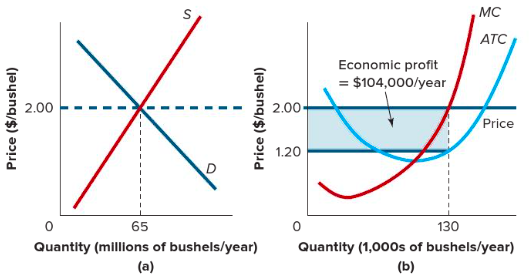
\includegraphics[scale=0.8]{Afsnit/Lektion3/Okonomiskprofit.png}
Her overskrider prisen offeromkostningerne af det det kræver at træde ind på markedet hvis det antages at alt udstyr der kræves er ledig til en konstant pris, og det er gratis at komme ind markedet. 
\end{eks}

I dette eksempel vil der komme flere og flere ind på markedet. Ved at der kommer flere udbydere på markedet vil udbudskurven flyttes mod højre og prisen vil falde. Hvis prisen falder, vil folk blive på markedet og måske endda komme ind på markedet indtil markedsprisen er lig de totale omkostninger. Når dette sker vil den økonomiske profit være lig 0. Det modsatte vil ske hvis prisen er under de totale omkostninger. Det er selvfølgelig ikke alle markeder hvor man bare kan skifte til og fra. Der kan være maskine eller arbejdskraft der ikke er mulig at skaffe og man kan derfor ikke skifte. Dette gør analysen noget mere kompleks. 

Hvis man antager at man bare kan gå ind i eller forlade kornmarkedet på ethvert tidspunkt betyder at kornproduktionen altid kan udvides eller reduceret på lang sigt til en pris på 1kr per bushel. Dette betyder at udbudskurven skal være en horisontal linje lig minimum af de totale omkostninger, 1kr per bushel. 

Ved prisen der er lig minimum af de totale omkostninger, vil hver udbyder have en økonomisk profit på 0. Dette er den langsigtede ligevægt. Det er også her til den bestemte pris at udbyderen oplever den maksimale profit og det er her køberne skal give det det koster at producere varen. 

\begin{eks} \textbf{} %Nyt eksempel
\newline
Hvis der for frisører og massører gælder at der er et økonomisk overskud på 0. Hvis der sker noget der sker noget så efterspørgselskurven for frisører forskydes til venstre og for massører forskydes til højre, vil der komme et nyt kortsigtet ligevægtspunkt for dem og prisen ændres. 

Da de begge startede med et økonomisk overskud på 0, vil frisøren opleve underskud og massøren overskud nu. Derfor vi frisører forlade faget og der vil komme flere massører til, dermed vil udbudskurverne flyttes mod venstre(frisør) og højre(massør). Dette vil ske indtil den langsigtede ligevægt nås. Det vil være den samme pris som der var ved udgangspunktet, men der vil være færre frisører og flere massører. 
\end{eks}

\subsubsection{The importance of free entry}
Hvis det ikke er muligt at træde ind i et marked hvor der er et økonomisk overskud vil markedet ikke gå mod langsigtede ligevægt. Dette kan skyldes \textbf{hindringer i at indgang}, fx copyright, lovmæssige krav og praktiske ting. På samme måde kan der være \textbf{hindringer i at forlade markedet}.

\subsection{Economic rent versus economic profit}
\textbf{Økonomisk leje} er forskellen mellem udbyderens reservationspris og salgsprisen. 

\begin{eks} \textbf{} %Nyt eksempel
\newline
Hvis der er 100 resturanter hvor af 99 af dem betaler deres kokke 30.000kr om året hvilket er det samme som de ville kunne tjene ved at lave noget andet. Den sidste koks mad er så godt at folk vil betale 50 procent mere for det end andre steder. Ejerne af de 99 resturanter tjener hver 300.000kr hvert år som er præcis det samme som deres normale profit. Da kunderne ved den sidste resturant er villige til at betale 50 procent mere, tjener resturanten 450.000kr om året. På lang sigt skal konkurrence sikre at kokken får 180.000kr om året. 30.000kr som de nomale kokke får og 150.000 ekstra fra den ekstra indtjening. Kokkens reservationspris er 30.000kr om året da det er det hun kan tjene i et andet fag og derfor er hendes økonomiske leje 150.000kr om året. Den økonomiske profit for ejerne af resturanten er 0. Resturanten ejer er nødt til at betal kokken de 180.000kr for eller er der andre der ville byde på kokken og det ville ske indtil der var nogen der bød 180.000. Efter dette ville det ikke kunne betale sig.
\end{eks}

\subsubsection{The invisible hand in action}
\textbf{How do cost-saving innovation affect economic profit in the short and long run?}:\\
Hvis der sker en forbedring som den økonomiske profit stiger vil der ske følgende. Hvis det kun er indenfor et enkelt lille firma denne forbedring sker, vil der ikke ske noget med markedsprisen og firmaet vil tjene mere. Når flere og flere firmaer får forbedringen vil udbudskurven forskydes nedad da marginal omkostningerne falder, og markedsprisen vil hermed falde. Derfor falder den økonomiske profit igen til det oprindelige. Den langsigtede udbudskurve vil tilsidst være forskudt ned og alle vil tjene deres normal profit. Hvis der er firmaer til denne tid der ikke har fået forbedringen endnu vil de få et økonomisk underskud. 

\subsection{The distinction between an equilibrium and a social optimum}
Når ligevægt er nået er der ikke mulighed for at optimere mere for individer. Det betyder ikke at det ikke er muligt at være bedre stillet når markedet ikke er i ligevægt. Nogle gange kan firmaer tjene meget ved at være de første til at gøre noget, fx købe en nye slags maskine. Det er formentlig nogen der virkelig har styr på markedet eller er heldig. 

\subsubsection{Smart for one, dumb for all}
Overskriften siger ligesom det hele....

\subsubsection{Market equilibrium and efficiency}
Når økonomer taler om \textbf{effektivitet} eller \textbf{Pareto effektivitet} har det en meget snæver teknisk mening. Når man siger at markedsligevægt er effektivt menes følgende: \textit{Hvis prisen og mængden er andet end ved ligevægtværdierne, vil man altid skade andre ved at hjælpe nogen}. Det er dermed effektivt ved at i ligevægt kan man hjælpe nogen uden at skade andre. Køber eller sælger er frustreret. Hvis prisen er over ligevægt vil det gavne alle hvis prisen faldt, da det vil komme tættere på alles reservationspris, derfor kan det ikke være effektivt at sælge over ligevægt. På samme måde kan det også kun blive bedre for begge parter hvis prisen stiger. Dermed kan det konkluderes at det i det frie marked gælder at det er mest effektivt i ligevægt. 

Dette holder dog kun hvis der er fuldkommen konkurrence, og opfylder andre restriktioner. Fx hvis udbudskurven ikke inkluderer alle omkostninger. Hvis en udvidelse af output resulterer i mere forurening vil koste mere end indikeret på markeds udbudskurven. Dermed vil ligevægt output være høj ineffektiv og ligevægts prisen være lav ineffektiv. Det kan også være at kurverne ikke får alle fordele med mm.

\textbf{Efficiency is not the only goal}: Ligevægt resultere i maksimal økonomisk overskud. Effektiv $\neq$ godt. Noget så simpelt som indkomst, kommer ind i spillet her. Når markedet for mælk er effektivt ved en pris på 8,50kr per liter, er det ikke alle der har råd til det. Sådan vil det være på mange markeder, at bare fordi det er effektivt er det ikke godt for alle. Nogle gange skal man lave regler for visse marked så man er sikker på at alle har en mulighed for at få noget. 

\textbf{Why efficiency should be the first goal}
Effektivitet er et mål da det hjælper os med at nå vores andre mål bedste/mest muligt. Ved ligevægt er det altid muligt at generere yderligere overskud.

\subsection{The cost of preventing price adjustments}
\subsubsection{Price ceilings}
Fx da priserne steg helt vildt i 70'erne pga stoppet af olielevering fra mellemøsten, lavede man i USA et loft på hvor meget olien måtte koste for at sikre at fattige familier ikke frøs ihjel i deres hus. Dette gør dog at der tit sker et fald i økonomisk overskud for udbyderne. Nedfor ses der 2 figurer den første viser uden et prisloft og den anden viser et prisloft på 1dollar/gallon. Beregn de blå og grønne arealer for at finde overskud for køber og udbyder.

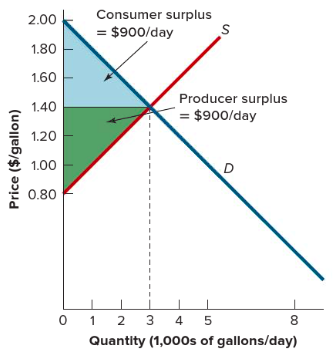
\includegraphics[scale=0.5]{Afsnit/Lektion3/loft1.png}

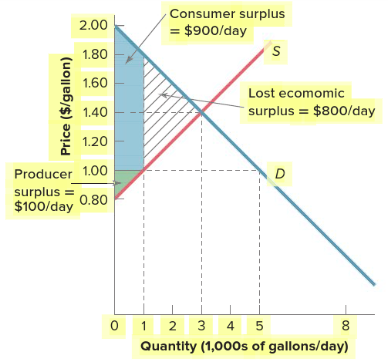
\includegraphics[scale=0.5]{Afsnit/Lektion3/loft2.png}

Ved lavere pris vil dem med mindre reservationspris købe mere end dem med højere reservationspris. Det vil ske da dem med højere reservationspris vil stadigvæk have et overskud hvis prisen bare stiger en smule. Derudover kan en reduktion i pris også gøre at folk vil gøre mere for at få fat i varen, fx stå i lange køer og stå tidligt op. 

Men hvorfor giver man ikke bare de fattige nogle flere penge istedet for at sætte et prisloft, som giver et større tab i total overskud. Udbydere vil nok være mere villig til at betale en smule mere i skat hvis de slipper for et stort tab. Disse skatter kunne bruges på at hæve indkomsten for de fattige som ville få stor gavn af det. Begge ville få mere gavn af dette og det er derfor man burde gøre det istedet for at indføre et prisloft. 
Det kan dog betyde at for fattige er det mindre attraktivt at arbejde, men det kommer i et andet kapitel.

\subsubsection{Price subsidies}
Regeringen kan sælge til en lavere pris end verdensprisen. Når de gør det kan der stadig ske et fald i det totale økonomiske overskud. Det sker da det er skattepenge der alligevel skal betale den "rabat" regeringen giver. Eks på side 196-197.

Alt i alt. Problemet er at fattige familier tjener for lidt. Den simpleste og bedste løsning bare at give dem flere penge. 

\subsubsection{Vigtigt fra forelæsningen}
Som revisor ser man på profit som egentlig profit(regenskabsmæssig profit). Økonomer ser også på offeromkostningerne(økonomisk profit). Offeromkostningerne kaldes normal profitten. 





